\setchapterpreamble[u]{\margintoc}
\chapter{硬件层面的解决方案}
\labch{hardware}

\setlength\parindent{2em} 本章将介绍本课题中硬件的设计思路、硬件主体与其它元器件的选材、电路规划与PCB印刷线路板的设计。包括电路实现方式、连接方式、工作流程以及对电路所做的兼容性、安全性、易修复性的优化。

\section{设计思路}

\setlength\parindent{2em} 本次研究最终要达到的目的是通过网络控制电路的通断,所以大概的方向就是将带有无线网络接收(或发射)功能的微控制单元(Microcontroller Unit, MCU;或称为单片机)\sidenote{微控制单元,是把中央处理器的频率与规格做适当缩减,并将内存、计数器、UART等周边接口,整合在单一芯片上,形成芯片级的计算机,为不同的应用场合做不同组合控制。\\以下称为单片机},或者是可以通过其他电路实现此功能的单片机进行编程,从而实现对电路的控制。
\par 具体来说,一般的小型单片机都有通用型之输入输出接口(GPIO),可用于控制电路。GPIO既可用于输入,亦可用于输出,但对与此研究项目来说,只会用到它的输出功能,即调整某些引脚电位的高低来对外部电路造成影响从而实现输出的目的。本研究项目所用的实现方法是通过改变GPIO的电位来造成外电路中部分电路的电位差从而使电流流过光电耦合器\sidenote{光电耦合器是以光为媒介传输电信号的一种电一光一电转换器件。它由发光源和受光器两部分组成。把发光源和受光器组装在同一密闭的壳体内,彼此间用透明绝缘体隔离。发光源的引脚为输入端,受光器的引脚为输出端,常见的发光源为发光二极管,受光器为光敏二极管、光敏三极管等等。}以控制另一部分电路的通断。将这一部分电路作为继电器的输入回路;在此之前,可以用一个金氧半场效晶体管来对电流方向进行管理和限制。
\par 大概的设计思路如此。除这种用单片机与无线网络实现之外,还可以用蓝牙、传感器、磁敏、光敏电阻等配合逻辑电路实现。但考虑到成本、技术要求,特别是便携程度与兼容性,最后选择了单片机用于此课题的研究与实践。

\section{选材与电路概念规划}

\setlength\parindent{2em} 由于本研究项目中对单片机的功能要求较为单一,所以选择了ESP8266-01S(以下简称为ESP01S)作为微控单元,其本身也可以作为无线网络模块连接与51单片机等通信。ESP01S的工作电压为3.3V。至于继电器,就选择常用的SRD-05VC-SL-C,其共有五个引脚,其中两个是线圈的引脚,另外三个分别是常闭端(NC)、常开端(NO)和公共端(COM)。其驱动电压为5V,最大允许10A,250V交流电通过,所以用来控制交流220V市电很合适。
\par 至此,所要设计的电路的输入与输出端有哪些,基本可以确定。除去天线以外,需要有一个电源输入以给单片机以及继电器电路供电。由于ESP01S的工作电压为3.3V,继电器控制电压为5V;所以总输入电压选择5V或者12V,这两种电压很容易获得,且可以通过降压来保证各个元件正常工作。最终确定为5V总电压,输入后通过LD1117芯片降成3.3V供予MCU(\reffig{normalconcept})。

\begin{figure*}[h!]
	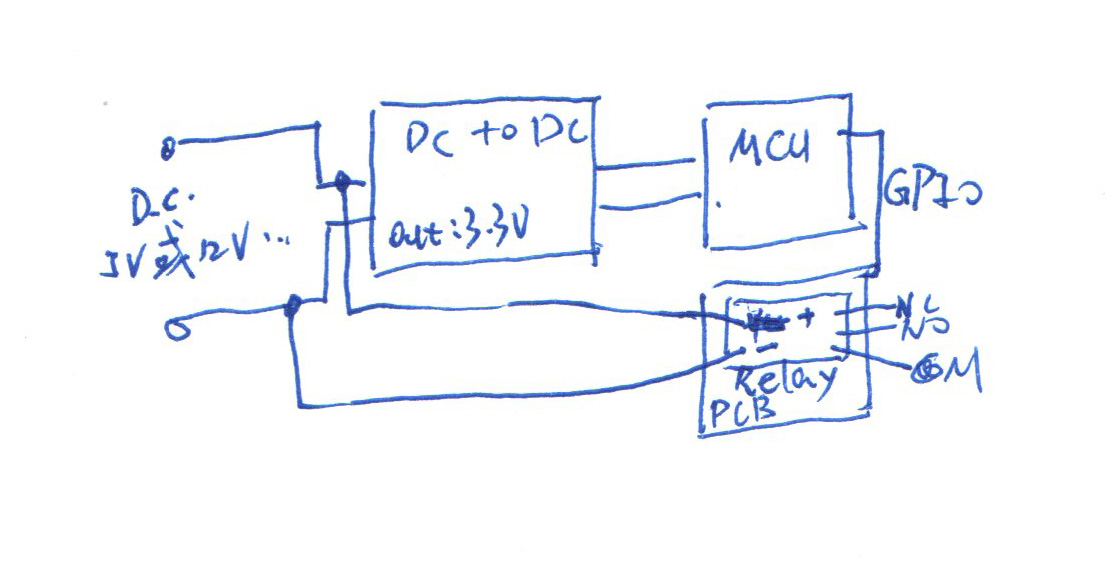
\includegraphics[width=\textwidth]{concept}
	\caption[concept]{电路的概念图}
	\labfig{normalconcept}
\end{figure*}

\begin{marginfigure}[-0.5cm]
	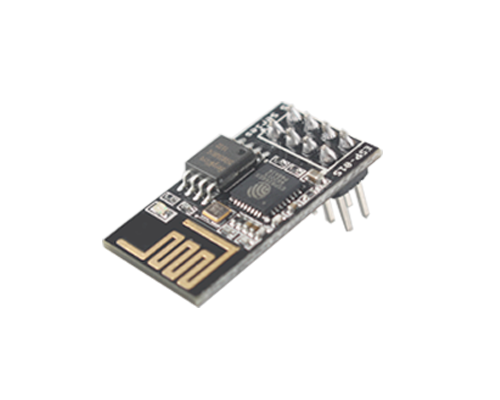
\includegraphics{esp01s}
	\caption[esp01s]{The ESP01S}
\end{marginfigure}

\begin{marginfigure}[0cm]
	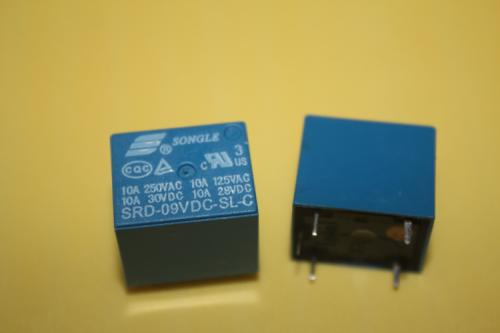
\includegraphics{relay}
	\caption[relay]{The SRD-05VC-SL-C}
\end{marginfigure}

%\begin{kaobox}[frametitle=To Do]
%Implement the \Option{justified} and \Option{margin} options. To be 
%consistent with the \KOMAScript\xspace style, they should accept a 
%simple switch as a parameter, where the simple switch should be 
%\Option{true} or \Option{false}, or one of the other standard values for 
%simple switches supported by \KOMAScript. See the \KOMAScript\xspace 
%documentation for further information.
%\end{kaobox}

\par 电路的大致概念如图\reffig{normalconcept}所示。输入电压为5V(可以通过USB供电),经过降压得到3.3V电压,供予MCU;继电器电路与降压芯片并联,得到5V电压;继电器电路与MCU之间通过GPIO通信。但图中还未给出具体细节,下一步就是对具体的电路进行规划与设计。\\
以下是本研究项目所用到的元器件:

\begin{itemize}
	\item ESP10S
	\item SRD-05VC-SL-C
	\item LD1117
	\item PC817光电耦合器
	\item 2n7002金氧半场效晶体管
	\item (发光)二极管数个
	\item 电容数个
	\item 电阻数个
	\item 电键
\end{itemize}

\section{电路图绘制}

\setlength\parindent{2em} 根据概念图,将LD1117的输入端和继电器线圈的一端与电源正极相连,其间连接一个1微法拉的电容接地用于滤波;出端再接一个100纳法拉的电容接地用于滤波;接地端连接负极。规定电源负极为电位零点,则LD1117输出端电压为3.3V,可直接供予ESP01S的VCC引脚。在ESP01S上,有一个标记为CH\_PD的引脚,这个引脚——从资料上看——是用来控制芯片的状态的,如果它是低电平,芯片处于关机状态;若是高电平,则芯片正常工作。于是将ESP01S的CH\_PD引脚连接至3.3V的供电,之间放置一个10kΩ的上拉电阻。
\par 为实现GPIO的控制目的,将GPIO与一个10kΩ的起保护作用的电阻串联,再使光电耦合器与一个470R电阻串联后与其并联,使得GPIO的电位变化可以对光电耦合器产生影响。光电耦合器的发射极与N沟道MOSFET\sidenote{金氧半场效晶体管(Metal-Oxide-Semiconductor Field-Effect Transistor, MOSFET)是一种可以广泛使用在模拟电路与数字电路的场效晶体管。MOSFET依照其“通道”(工作载流子)的极性不同,可分为“N型”与“P型” 的两种类型,通常又称为NMOSFET与PMOSFET,其他简称上包括NMOS、PMOS等。}的栅极相连,若光电耦合器通路,MOSFET的源极与漏极也导通,继电器线圈的一端就会接地,与另一端产生5V的电位差,线圈通电,继电器工作。从而实现通过GPIO的电位变化来控制继电器通断的目的。最后用一个发光二极管与线圈并联作为指示灯;设置好RESET电建用于MCU的复位,电路的总体设计基本上就完成了。完整的电路(5V的供电未给出)如图\reffig{normalcircuit}所示:

\begin{figure*}[h!]
	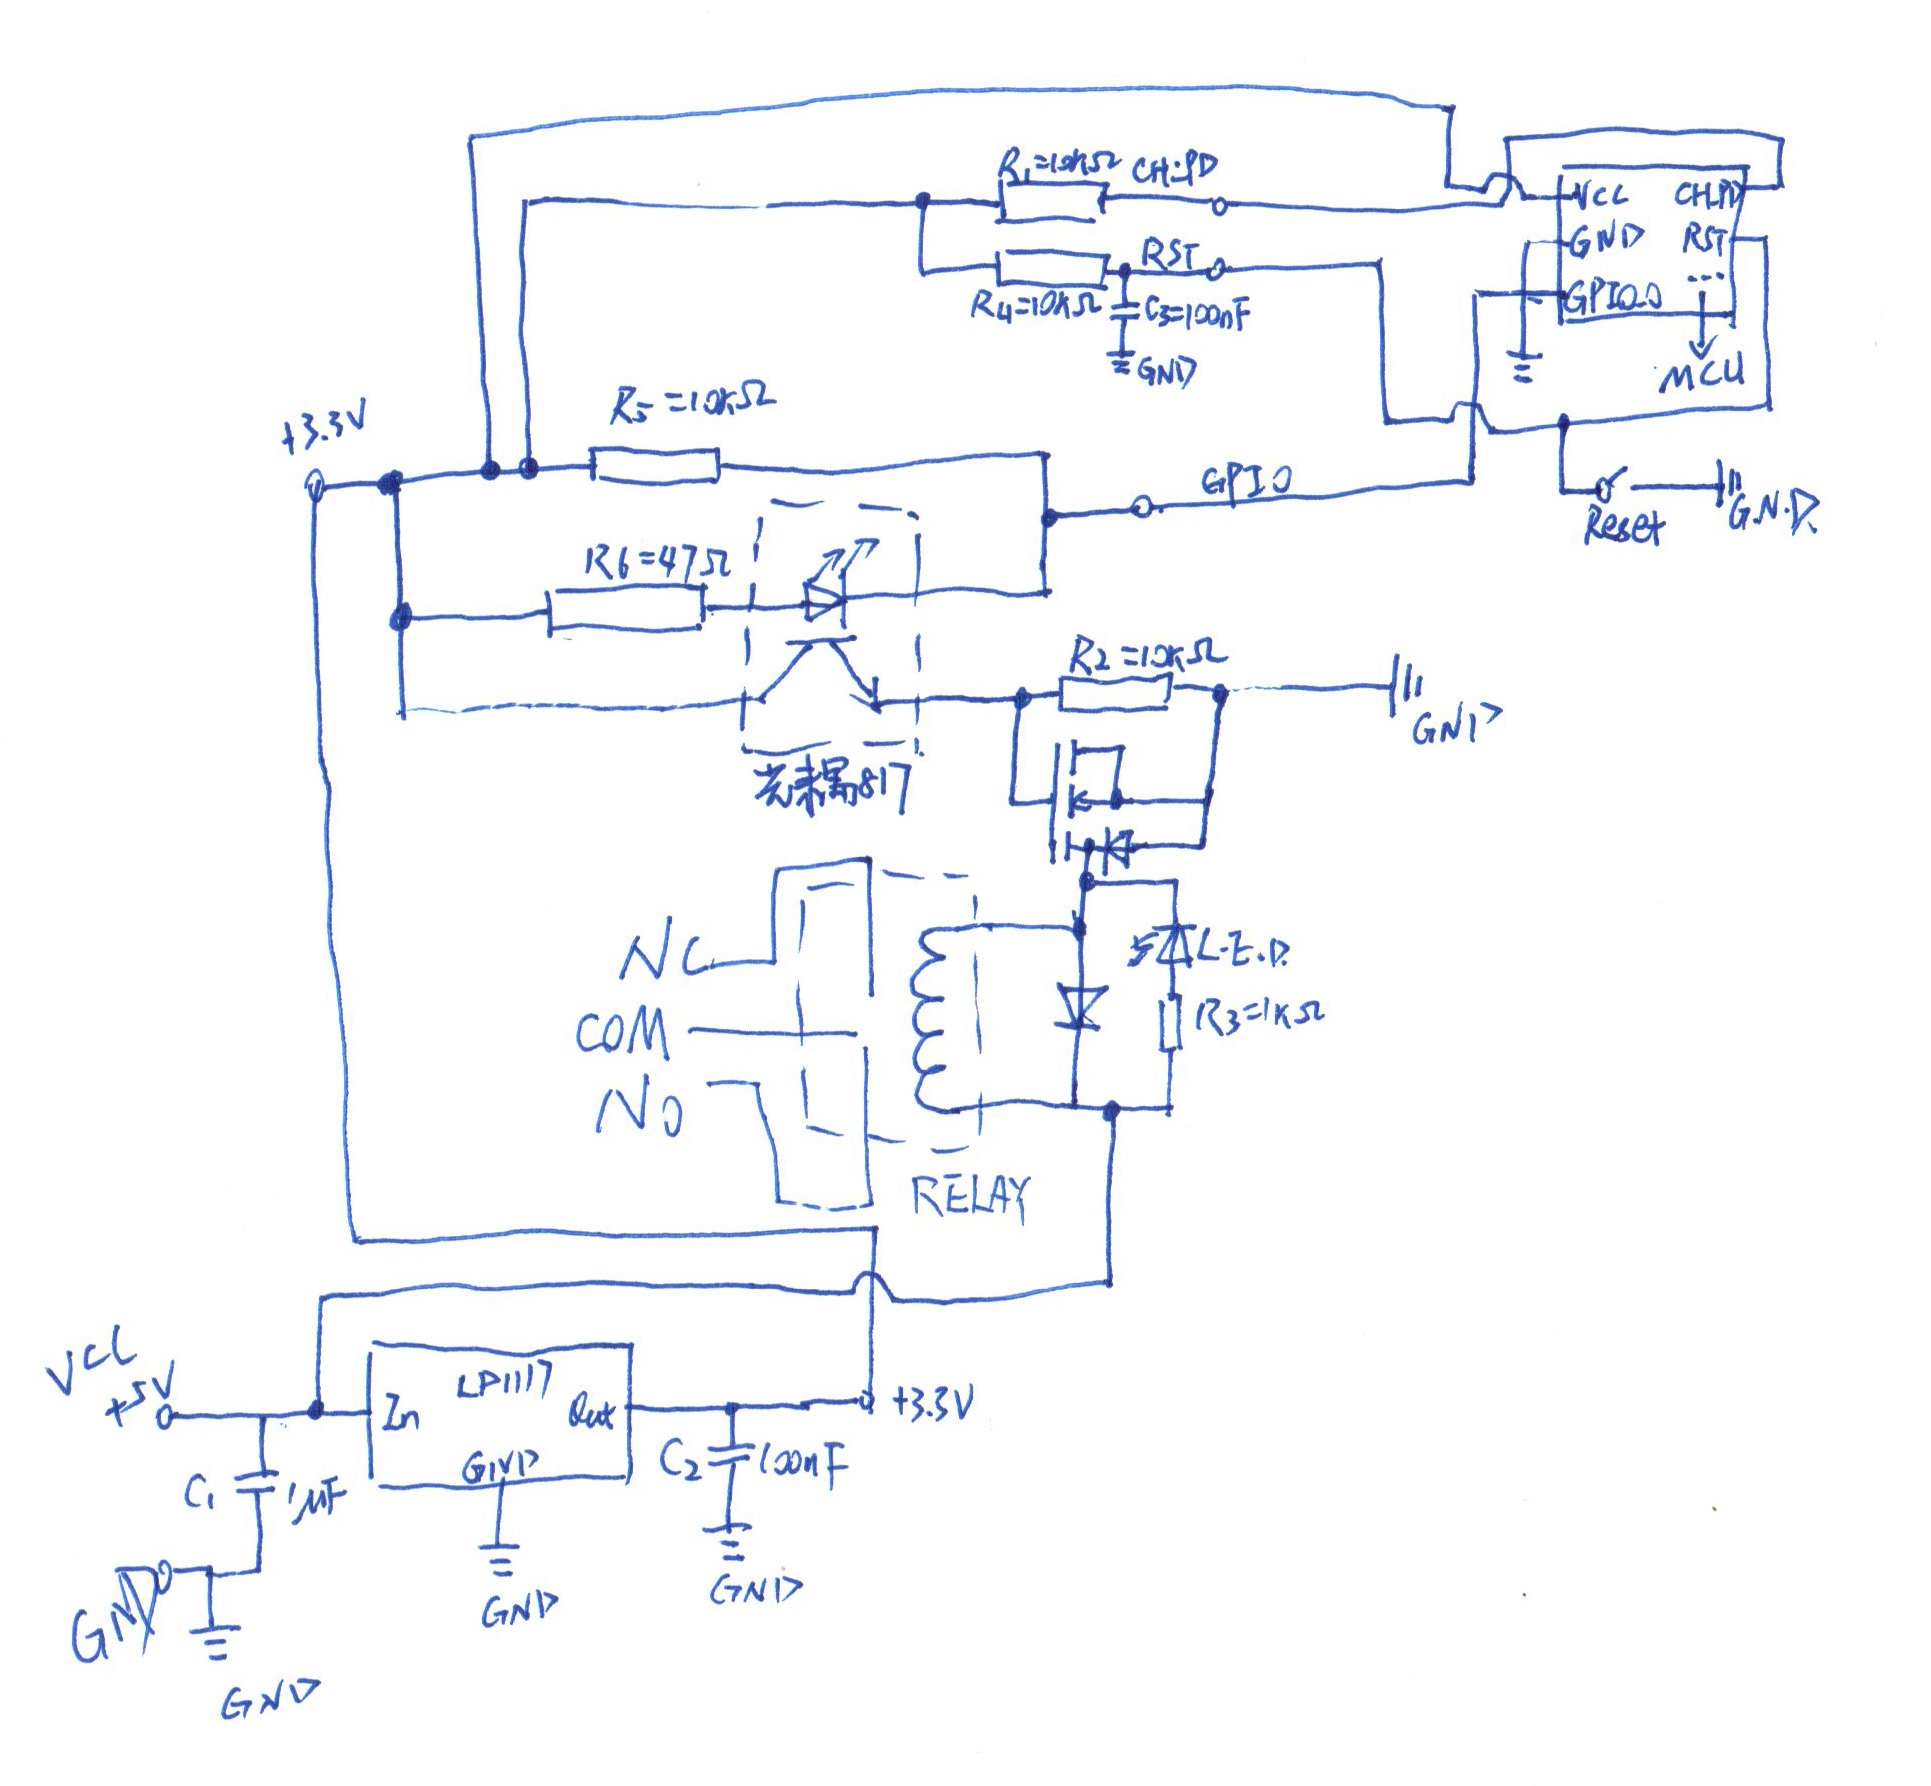
\includegraphics[width=\textwidth]{circuit}
	\caption[circuit]{完整的电路图(5V的供电未给出)}
	\labfig{normalcircuit}
\end{figure*}

\section{依照电路图绘制原理图及设计PCB}

\setlength\parindent{2em} 依照已经绘制完成的电路图,进行PCB印刷线路板的设计。首先需要绘制原理图。上面的电路图大致可以分为四部分:供电部分、单片机部分、光电耦合器部分和继电器部分。依照这个,将电路图中的节点拆分,可以得到原理图。
\par 实际制作时,输入输出接口用端子座实现,所有的接地处,也就是电位为零处,统一接至PCB的地平层。
\par 原理图如图\reffig{normalschematic}所示:
\begin{figure*}[h!]
	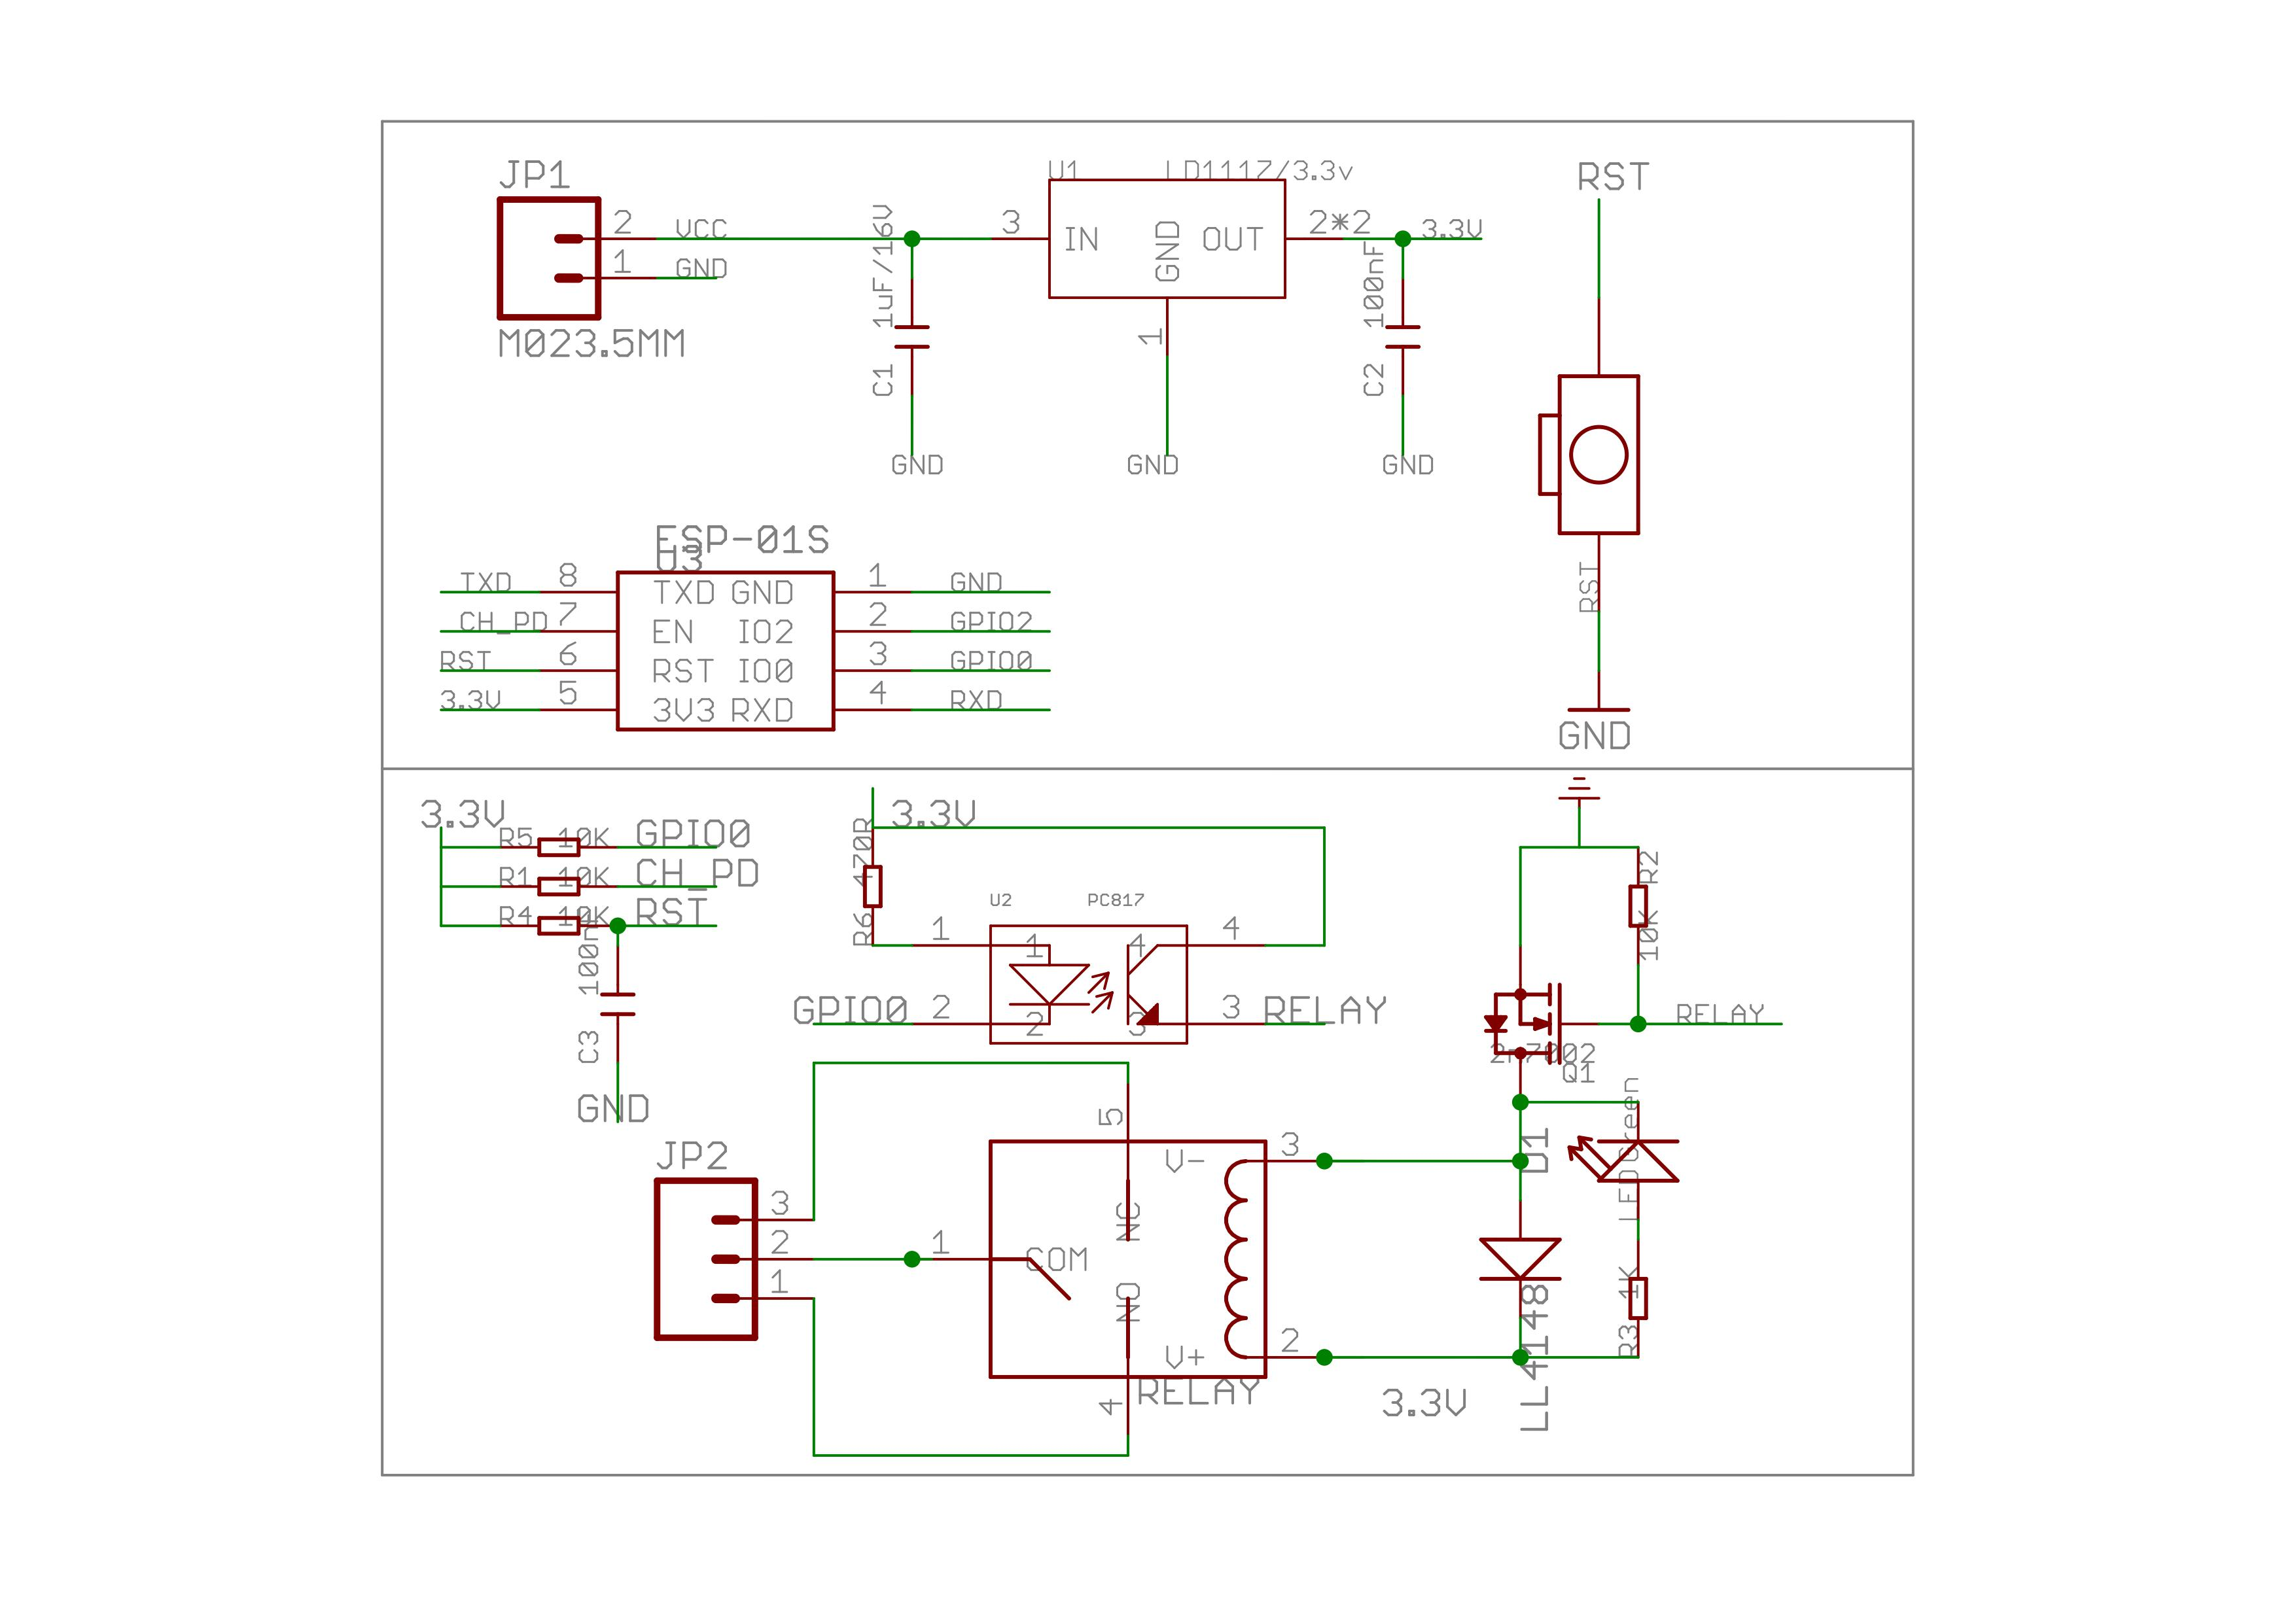
\includegraphics[width=1.5\textwidth]{schematic}
	\caption[schematic]{电路的原理图}
	\labfig{normalschematic}
\end{figure*}